\documentclass[tikz]{standalone}

\usepackage{amsmath}

\usetikzlibrary{
  math,
  positioning,
  shapes.geometric,
}

\newcommand{\given}[1][]{\:#1\vert\:}
\newcommand{\saf}[2]{
  p(X_{#1} \given Z_{#1} = #2)
}
\newcommand{\sfs}[1]{
  \widehat{\phi}^{(#1)}
}
\newcommand{\bsfs}[1]{
  \widehat{\psi}^{(#1)}
}
\newcommand{\post}[3]{
  p(Z_{#1} = #2 \given X_{#1}, \sfs{#3})
}

\begin{document}

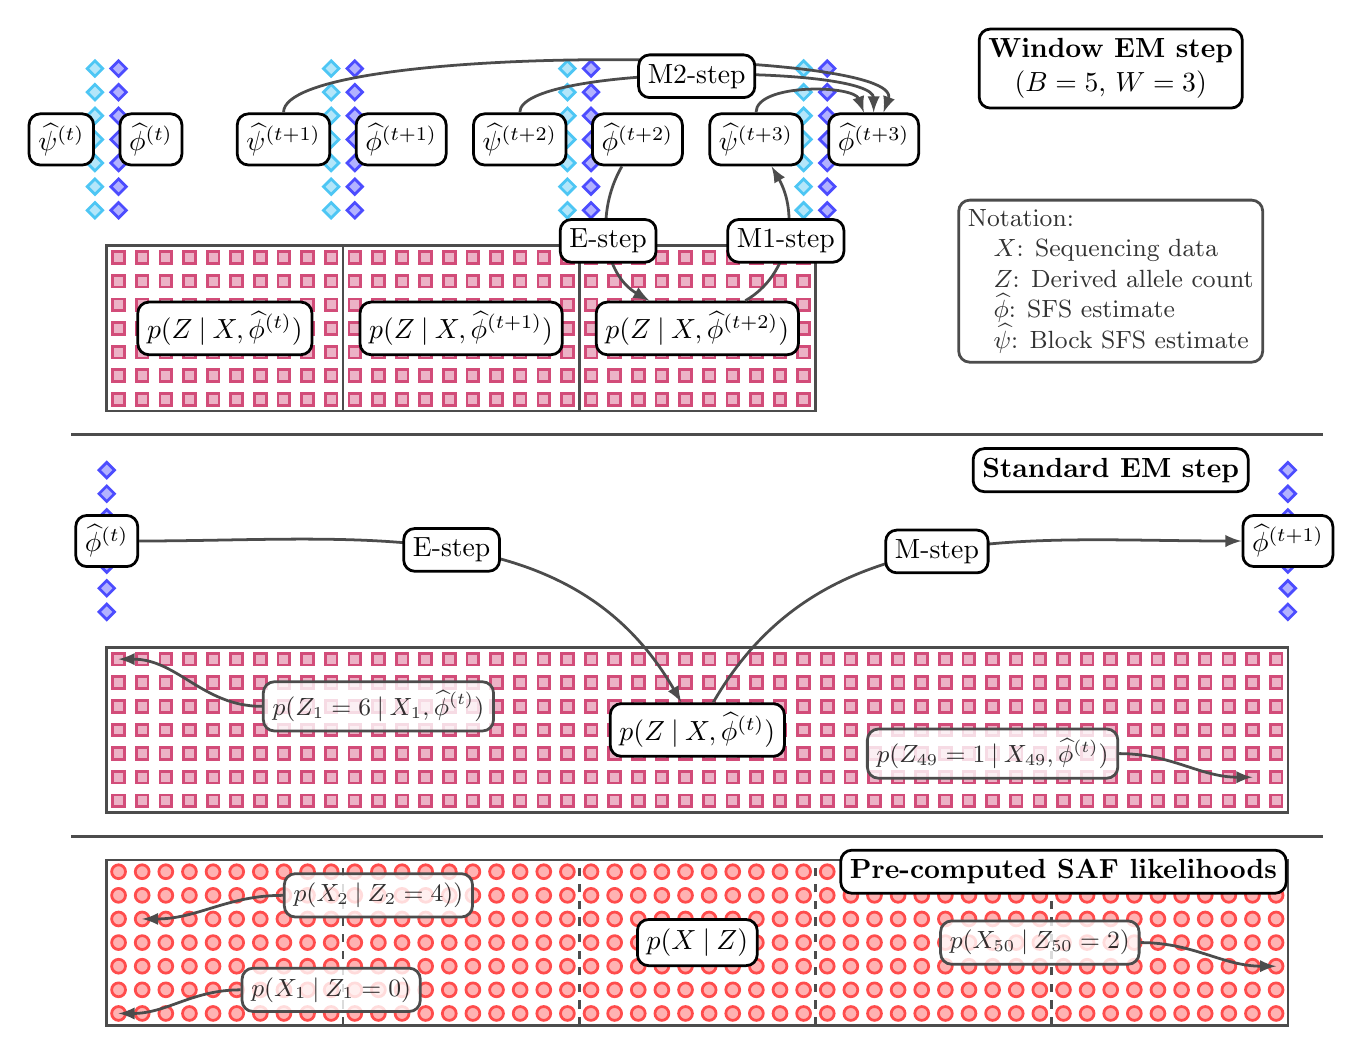
\begin{tikzpicture}[
  scale=0.3,
  element/.style n args={1}{
    draw,
    line width=1pt,
    inner sep=0pt,
    color=#1!70,
    fill=#1!30,
    minimum size=5pt,
  },
  saf/.style={
    element={red},
    circle,
  },
  post/.style={
    element={purple},
  	regular polygon,
  	regular polygon sides=4,
    minimum size=6pt,
  },
  sfs/.style={
    element={blue},
    diamond,
    minimum size=6pt,
  },
  bsfs/.style={
    element={cyan},
    diamond,
    minimum size=6pt,
  },
  box/.style={
    draw=black!70,
    rounded corners,
    line width=1pt,
    text=black,
    fill=white,
  },
  big box/.style={
    box,
    draw=black,
    font={\normalsize},    
  },
  small box/.style={
    box,
    fill opacity=0.8,
    font={\small},
  },
  arrow/.style={
    -latex,
    draw=black!70,
    line width=1pt,
  },
  sep/.style={
    draw=black!70,
    %dashed,
    line width=1pt,
  },
  block/.style={
    draw,
    black!70,
    line width=1pt,
  },
]
  \tikzmath{
    \M = 50;
    \N = 3;
    \2N = 2 * \N;
    \B = 10;
    \W = 3;
    \xmid = (\M + 1) / 2;
    \ymid = \N;
  }

  %%%%%%%%%%%%%%%%%%%% SAF %%%%%%%%%%%%%%%%%%%%

  \foreach \x in {1,...,\M} {
    \foreach \y in {0,...,\2N} {
      \node[saf] at (\x,\y) {};
    }
  }

  \draw[block] (0.5,-0.5) rectangle ++(\M,{\2N + 1});

  \foreach \b in {2,...,5} {
    \tikzmath {
      \blockxstart = (\b - 1) * \B + 1;
    }

    \draw[block, dashed] ({\blockxstart - 0.5},-0.5) to 
      ({\blockxstart - 0.5},{\2N + 0.5});
  }


  \node[big box] at (\xmid,\ymid) {$p(X \given Z)$};

  \node[small box] (a) at (10, 1) {$\saf{1}{0}$};
  \draw[arrow,out=180,in=0] (a) to (1, 0);

  \node[small box] (b) at (12, 5) {$\saf{2}{4})$};
  \draw[arrow,out=180,in=0] (b) to (2, 4);

  \node[small box] (c) at (40, 3) {$\saf{50}{2}$};
  \draw[arrow,out=0,in=180] (c) to (50, 2);

  % Separator
  \path[sep] (-1,{\2N + 1.5}) -- ({\M + 2},{\2N + 1.5});

  \node[big box] at (41,\2N) {\textbf{Pre-computed SAF likelihoods}};

  %%%%%%%%%%%%%%%%%%%% STANDARD EM %%%%%%%%%%%%%%%%%%%%

  \tikzset{shift={(0,{\2N + 3})}}

  \foreach \x in {1,...,\M} {
    \foreach \y in {0,...,\2N} {
      \node[post] at (\x,\y) {};
    }
  }

  \draw[block] (0.5,-0.5) rectangle ++(\M,{\2N + 1});

  \node[big box] (post) at (\xmid,\ymid) {$p(Z \given X, \sfs{t})$};

  \node[small box] (a) at (12, 4) {$\post{1}{6}{t}$};
  \draw[arrow,out=180,in=0] (a) to  (1, 6);

  \node[small box] (b) at (38, 2) {$\post{49}{1}{t}$};
  \draw[arrow,out=0,in=180] (b) to (49, 1);

  \tikzset{shift={(0,{\2N + 2})}}

  \foreach \y in {0,...,\2N} {
    \node[sfs] at (0.5,\y) {};
  }

  \node[big box] (sfs) at (0.5,\ymid) {$\sfs{t}$};

  \foreach \y in {0,...,\2N} {
    \node[sfs] at ({\M + 0.5},\y) {};
  }

  \node[big box] (newsfs) at ({\M + 0.5},\ymid) {$\sfs{t + 1}$};

  \draw[arrow,out=0,in=120] (sfs) to node[big box] {E-step} (post);
  \draw[arrow,out=60,in=180] (post) to node[big box] {M-step} (newsfs);

  \node[big box] at (43,\2N) {\textbf{Standard EM step}};

  \path[sep] (-1,{\2N + 1.5}) -- ({\M + 2},{\2N + 1.5});

  %%%%%%%%%%%%%%%%%%%% Window EM %%%%%%%%%%%%%%%%%%%%

  \tikzset{shift={(0,{\2N + 3})}}

  \tikzmath{
    \BW = \B * \W;
  }

  \foreach \x in {1,...,\BW} {
    \foreach \y in {0,...,\2N} {
      \node[post] at (\x,\y) {};
    }
  }

  \foreach \b/\t in {1/t,2/t+1,3/t+2,4/t+3} {
    \tikzmath {
      \blockxstart = (\b - 1) * \B + 1;
      \blockxmid = \blockxstart + (\B - 1) / 2;
      \sfsxstart = \blockxstart - 1;
      \sfsystart = \2N + 2;
    }

    \ifnum\b<4
      \coordinate (blocklowerleft) at ({\blockxstart - 0.5},-0.5);
      \draw[block] (blocklowerleft) rectangle ++(\B,{\2N + 1});
  
      \coordinate (blockmid) at (\blockxmid,\ymid);
      \node[big box] (post-\b) at (blockmid) {$p(Z \given X, \sfs{\t})$};
    \else
    \fi
  
    \foreach \y in {0,...,\2N} {
      \tikzmath {
        \sfsy = \sfsystart + \y;
      }
      \node[bsfs] at (\sfsxstart,\sfsy) {};
      \node[sfs] at (\blockxstart,\sfsy) {};
    }

    \coordinate (sfsmid) at (\sfsxstart,{\sfsystart + \N});
    \node[big box,anchor=east] (sfs-\b) at (sfsmid) {$\bsfs{\t}$};

    \coordinate (bsfsmid) at (\blockxstart,{\sfsystart + \N});
    \node[big box,anchor=west] (bsfs-\b) at (bsfsmid) {$\sfs{\t}$};
  }

  \draw[arrow,out=240,in=150] (bsfs-3) to node[big box] {E-step} (post-3);
  \draw[arrow,out=30,in=300] (post-3) to node[big box] {M1-step} (sfs-4);

  \draw[arrow,out=90,in=70,looseness=0.3] (sfs-2) to (bsfs-4);
  \draw[arrow,out=90,in=90,looseness=0.35] 
    (sfs-3) to node[big box] {M2-step} (bsfs-4);
  \draw[arrow,out=90,in=110,looseness=0.7] (sfs-4) to (bsfs-4);

  \node[big box] at (43,{2 * \2N + 2}) 
    {
      \shortstack{
        \textbf{Window EM step} \\
        ($B=5$, $W=3$)
      }
    };

  %%%%%%%%%%%%%%%%%%%% Notation %%%%%%%%%%%%%%%%%%%%

  \node[small box,align=left] at (43,{\2N - 1}) 
    {
      Notation: \\
      %
      $\quad X$: Sequencing data \\
      $\quad Z$: Derived allele count \\
      $\quad \widehat{\phi}$: SFS estimate \\
      $\quad \widehat{\psi}$: Block SFS estimate
    };
\end{tikzpicture}

\end{document}